\section{Evaluation}
In their original work, \citeauthor{10.1007/978-3-030-15986-3_19} identified four pitfalls and their effects in the collected datasets. This section examines three major pitfalls: Redirects, Object Sizes, and Byte Index more closely using both data from the original dataset and the newly collected measurements. 

\subsection{Redirects}
As mentioned in Section \ref{sec:background}, \citeauthor{10.1007/978-3-030-15986-3_19} makes the observation that initial redirects can increase PLT substantially. As seen in Figure \ref{fig:plot_redirects}, the dataset provided in the original paper also makes the more specific observation that this effect is especially pronounced for short page loads. While the new measurements / dataset does confirm that initial redirects can have a large effect on PLT, the difference in short load times is less pronounced. 

The percentage of redirects taking an abnormally long time remained relatively constant between both datasets: In the original dataset, 11.20482\% (Firefox Datasets Only: 13.9249\%) of redirects take more than one second; The new dataset provides a similar result with 12.34043\% of redirects taking more than one second. The number of redirects increased slightly in the new dataset: in the original dataset, the mean number of redirects in measurements performed by Firefox using Marionette was 1.258; the new dataset's measurements produced a mean number of redirects of 1.393. The new dataset confirms that redirects can have an impact on PLT, albeit less significant than in the original dataset. The suggestion for papers to make a conscious choice regarding the inclusion or exclusion of redirects in timing is, therefore, still valid.

\subsection{Object Sizes}
In the original paper, \citeauthor{10.1007/978-3-030-15986-3_19} compare the object sizes for all pages (including those transferred over encrypted connections). In Figure \ref{fig:relative_byte_index}, the object size differences across the different data sources (HAR file body size, Content-Length header in HAR file, and Resource Timings) are displayed. Content-Length header (taken from browser) is used as a close approximation for a baseline. In the original dataset (Firefox Only): Resource timings, HAR body size, and HAR Content-Length provide the exact same object size as the baseline in 42.5\%, 91.3\%, 42.4\% of cases respectively. These percentages are drastically different in the new dataset for both HAR body size and HAR Content-Length: Only 0.02\% and 0.88\% match the baseline exactly. Resource Timings, however, provide a relatively accurate measure of object sizes and math the baseline in 43.88\% of all cases.

This data, as shown in Figure \ref{fig:absolute_byte_index}, clearly shows that the new measurements do not confirm the conclusion that Content-Length found in HAR files is the most accurate measure of object sizes. The new dataset instead leads to the conclusion that object sizes provided by Resource Timings provide the most accurate approximation of total object size. The fact that it is only an exact match in fewer than half of all cases, however, does not make it an ideal measure. The difference between HAR Content-Length is very strongly concentrated in one range between 100 and 1000 bytes, where over 90\% of measurements can be found (see Figure \ref{fig:new_absolute_byte_index}); this suggests that there is a consistent reason for this difference and that it can be accounted for (e.g. with a constant offset). 

\begin{figure}
 \centering
 \begin{subfigure}{\linewidth}
		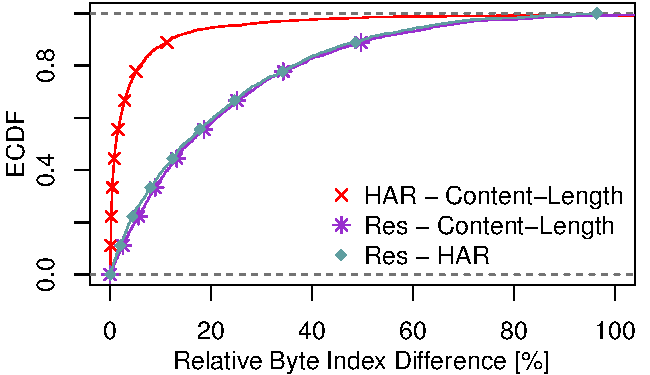
\includegraphics[width=\linewidth]{New_Plots/ecdf_rel_object_byte_index.pdf}
	\caption{New Measurements}
	\label{fig:new_relative_byte_index}
\end{subfigure}\par\medskip
 \begin{subfigure}{\linewidth}
		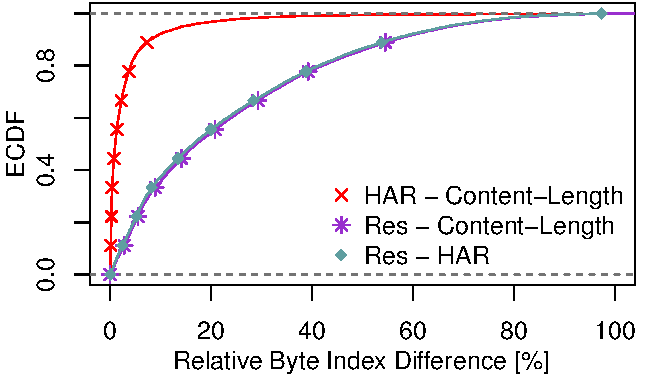
\includegraphics[width=\linewidth]{Firefox Plots/ecdf_rel_object_byte_index.pdf}
	\caption{Original Measurements (Firefox Only)}
	\label{fig:orig_firefox_relative_byte_index}
\end{subfigure}\par\medskip
 \begin{subfigure}{\linewidth}
		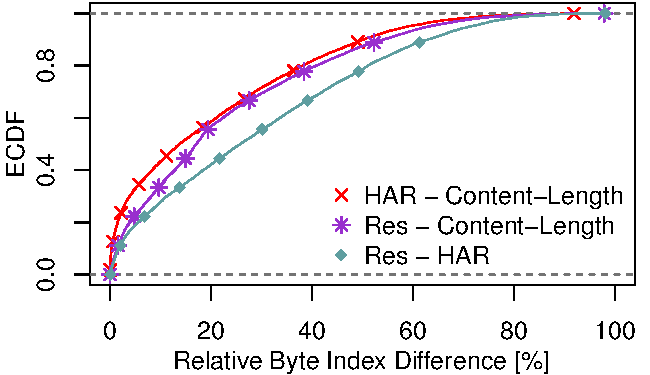
\includegraphics[width=\linewidth]{Chrome_Plots/ecdf_rel_object_byte_index.pdf}
	\caption{Original Measurements (Chrome Only)}
	\label{fig:orig_chrome_relative_byte_index}
\end{subfigure}
\caption{Byte index: difference due to data source}
\label{fig:relative_byte_index}
\end{figure}

\subsection{Object Count \& Byte Index}
In the original paper, \citeauthor{10.1007/978-3-030-15986-3_19} found that not only do object sizes differ significantly by data source but also object counts. In the original Alexa 1000 dataset, object counts for the same web pages differed between HAR files and Resource Timings by at least 7 objects. Figure \ref{fig:relative_byte_index} shows the relative difference between Byte Index for the same page load using HAR body size, Resource Timings body size and the Content Length header. As observed in the original measurements (Firefox Only), the Byte Index is close to identical for Content-Length and HAR body size; this observation is confirmed in the new measurements, as seen in Figure \ref{fig:new_relative_byte_index}. 

The results for Chrome, as seen in Figure \ref{fig:orig_chrome_relative_byte_index}, show that the Byte Index for both Resource Timings and HAR differed significantly from that of Content-Length. Unfortunately, due to the difficulties described in \ref{sec:scripts} it was not possible to confirm these findings using new measurements in Chrome. Thus, the conclusion of the original paper that resource timings do not include all objects of a web page is confirmed by the new dataset for Firefox.